\chapter{$P_N$-Method}
%
\label{sec:pnmethod}

The $P_N$-method is a deterministic method for computing light transport in a participating media. It is based on the spherical harmonics discretization of the radiative transfer equation and its related quantities in angular domain. The method has its origins in astrophysics and is also popular in nuclear sciences and medical science. It came up in the field of computer graphics only in so far that Kajia~\cite{Kajiya84} brushed over the theory, but did not give any details on implementation or how to solve it. In fact, as Max~\cite{Max95} pointed out, it is not clear if Kajiya succeeded at all at applying the method, as all of the results in his paper were produced with a simpler method\footnote{\cite{Max95} p.4: \emph{``[...] Kajiya attempted to solve these equations for the case of isotropic scattering, but it is unclear whether he succeeded, since all the pictures in \cite{Kajiya84} were produced by the simpler 'slab' method.[...]"}}. This doubt is further strengthened by results in this thesis, which show that a straight forward finite difference discretization of the $P_N$-equations produces unuseable results, due to oscillation artifacts in the solution. 
\TD{reference for pn method in astrophysics, neutron transport, medical sciences etc.}

In this chapter, we will give a thorough derivation of the $P_N$-theory. The first section introduces the spherical harmonics expansion and important properties. Then the complex-valued $P_N$-equations are derived in section~\ref{sec:pn_cvalued}. The fact, that the radiance field is positive in every direction can be used to cut the number of unknowns in half. This is done by using the real-valued $P_N$-equations. In section~\ref{sec:pn_rvalued}, a very compact form of the real-valued $P_N$-equations is derived, which has not been given anywhere else in the literature before. After a short note on two-dimensional problems in section~\ref{sec:pn_2d}, The chapter continues by introducing a new method for solving the $P_N$-equations (section~\ref{sec:pn_solver}) and closes by discussing its integration into a rendering framework and giving results (section~\ref{sec:pn_results}).

% ============================================================
\section{Spherical Harmonics}
\label{sec:sh}

Spherical harmonics are the Fourier series for the sphere, and are an important tool for solving numerical problems involving the spherical domain. They are often derived as eigensolutions to the surface Laplacian, which is the analog to developing the Fourier series as eigensolutions of the operator $(d/dx)^2$ on a finite line with the boundary conditions that $y$ and $dy/dx$ match at the two ends (see Riley et al.~\cite{Riley2006}). The result of this derivation are complex-valued functions $\SHBC$, which are defined as:
\begin{align}
\label{eq:sh_definition}
\SHBC^{l,m}(\theta, \phi)=
\begin{cases}
C^{l,m}e^{im\phi}P^{l,m}\left(\operatorname{cos}\theta\right), & \text{for $m\ge0$}\\
\left(-1\right)^m\overline{\SHBC^{l\left|m\right|}}(\theta, \phi), & \text{for $m<0$}
\end{cases}
\quad ,
\end{align}
where $P^{l,m}$ are the associated Legendre polynomials. While those can be defined in many different ways, the most numerically robust way to evaluate them is by using the following set of recurrence relations (Press et al.~\cite{Press07}):
\begin{align}
P^{0,0}\left(\operatorname{cos}\theta\right) &=
1
\  ,
\nonumber
\\
P^{m,m}\left(\operatorname{cos}\theta\right) &=
\left(2m-1\right)!!\left(1-\operatorname{cos}^2\theta\right)^\frac{m}{2}
\  ,
\nonumber
\\
P^{m+1,m}\left(\operatorname{cos}\theta\right) &=
\operatorname{cos}\theta\left(2m+1\right)P^{m,m}\left(\operatorname{cos}\theta\right)
\ 
\nonumber
\\
P^{l,m}\left(\operatorname{cos}\theta\right) &=
\frac{\operatorname{cos}\theta\left(2l-1\right)}{l-m}
P^{l-1,m}\left(\operatorname{cos}\theta\right)
-
\frac{l+m-1}{l-m}
P^{l-2,m}\left(\operatorname{cos}\theta\right)
\  .
\label{eq:sh_Plm}
\end{align}
The factor $C^{l,m}$ in equation~\ref{eq:sh_definition} is defined as
\begin{align}
\label{eq:sh_definition_C}
C^{l,m}=(-1)^m\sqrt{\frac{2l+1}{4\pi}\frac{(l-m)!}{(l+m)!}}
\end{align}
Since spherical harmonics are used in many different fields, their definition can vary and one has to be careful, when comparing them across literature. This concerns the $(-1)^m$ factor in particular, which is called the Condon-Shortley phase. Sometimes, this factor is part of the definition of the associated Legendre polynomial $P^{l,m}$ and therefore does not appear in $C^{l,m}$. More importantly, the definition of $C^{l,m}$ depends on how the spherical harmonics are expected to be normalized.
\newline
\begin{figure}[h]
\centering
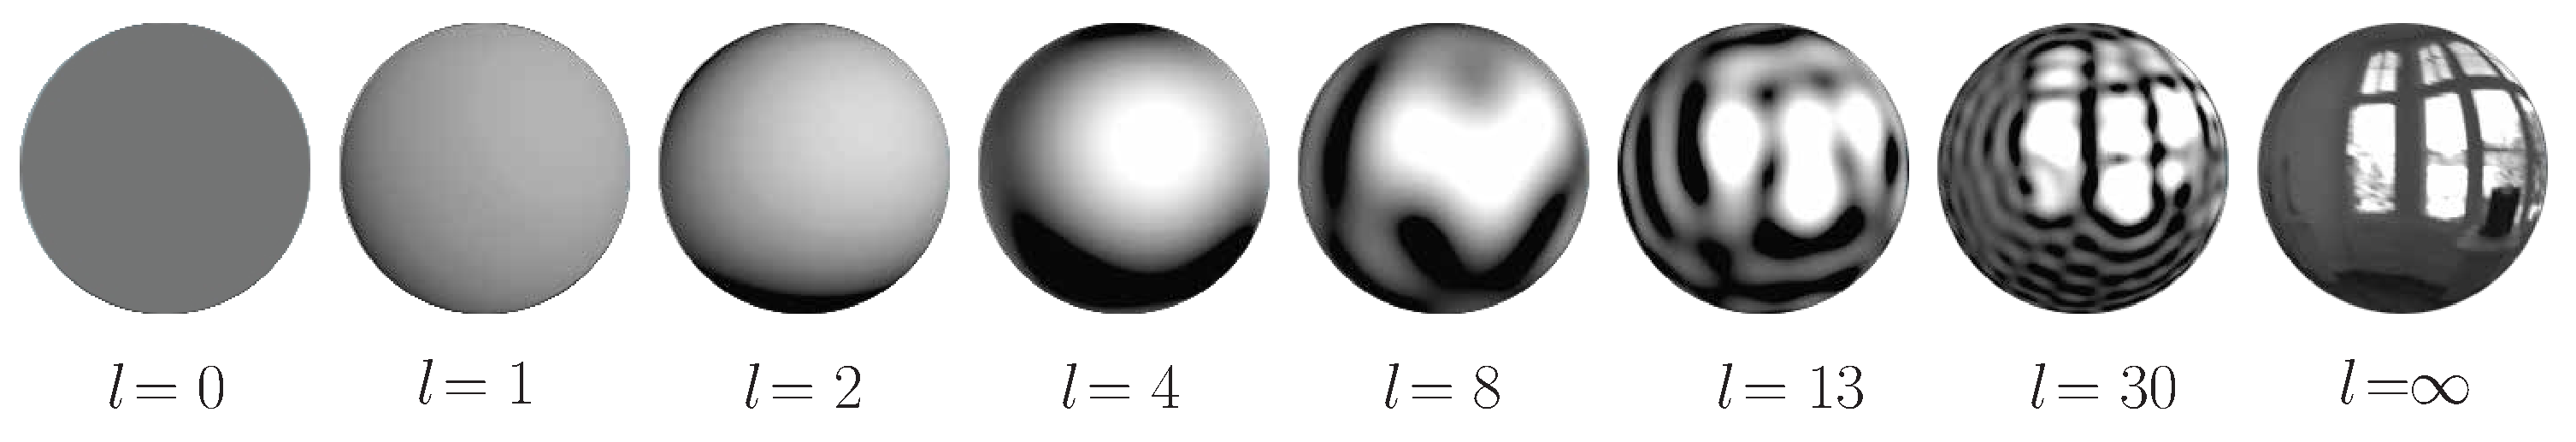
\includegraphics[width=\columnwidth]{04_pn_method/figures/fig_sph_frequencies.pdf}
\caption{Approximating a spherical function using spherical harmonics with increasing truncation order (from left to right). Like with the Fourier-transform, higher truncation order allows capturing higher frequencies.}
\label{fig:sh_vis}
\end{figure}


%\begin{figure}[h]
%\centering
%\begin{subfigure}{0.31\columnwidth}
%%\includegraphics[width=\columnwidth]{images/checkerboard2d_p1_neumann_staggered_starmap.png}
%%spherical harmonics basis function hierarchy in 2d
%\missingfigure{see comment}
%\caption{TODO}
%\label{fig:sh_vis_1}
%\end{subfigure}
%\hspace{0.01\columnwidth}
%\begin{subfigure}{0.31\columnwidth}
%%\includegraphics[width=\columnwidth]{images/checkerboard2d_p1_neumann_staggered.png}
%%some environment map and truncated reconstruction in 2d
%\missingfigure{see comment}
%\caption{TODO}
%\label{fig:sh_vis_2}
%\end{subfigure}
%\hspace{0.01\columnwidth}
%\begin{subfigure}{0.31\columnwidth}
%%\includegraphics[width=\columnwidth]{images/checkerboard2d_p1_neumann_staggered.png}
%%the hierarchy for the reconstruction with weights
%\missingfigure{see comment}
%\caption{TODO}
%\label{fig:sh_vis_3}
%\end{subfigure}%
%\caption{TODO}
%\label{fig:sh_vis}
%\end{figure}

\subsubsection*{Normalization and Orthogonality}

The coefficient $C^{l,m}$ has been defined as such that the spherical harmonics function $\SHBC$ scales to the unit norm
\begin{align}
\label{eq:sh_normalization}
\norm{\SHBC^{l,m}} = \sqrt{\left<\SHBC^{l,m}, \SHBC^{l,m}\right>} = 1
\ .
\end{align}
Other spherical harmonics definitions use a different constant (e.g. $4\pi$) and therefore arrive at different $C^{l,m}$. Since the spherical harmonics functions $\SHBC$ are complex-valued functions on the unit sphere, they are elements of the Hilbert space, for which the inner product is defined as:
\begin{align}
\label{eq:sh_inner_product}
\left<f,g\right> = \int_\Omega f\left(\vec{\omega}\right)\overline{g}\left(\vec{\omega}\right)\ud\vec{\omega}
\end{align}
with $\overline{g}$ being defined as the complex conjugate of $g$ (Folland~\cite{Folland92}).

The spherical harmonics functions form a orthogonal family and thus result in:
\begin{align}
\left<\SHBC^{l_1, m_1},\SHBC^{l_2, m_2}\right>
=
0
\ ,\quad\text{ for } l_1 \ne l_2 \text{ and } m_1 \ne m_2
\end{align}
The properties of normalization (equation~\ref{eq:sh_normalization}) and orthogonality (equation~\ref{eq:sh_orthogonality}) give
\begin{align}
\label{eq:sh_orthogonality}
\left<\SHBC^{l_1, m_1},\SHBC^{l_2, m_2}\right>=
\int_{\Omega} \SHBC^{l_1m_1}\left(\vec{\omega}\right) \overline{\SHBC^{l_2m_2}}\left(\vec{\omega}\right) \mathbf{d}\vec{\omega} = \delta_{l_1m_1}\delta_{l_2m_2}
\ .
\end{align}

\subsubsection*{Projection and Reconstruction}

Because the spherical harmonics are orthonormal, a spherical functional $f\left(\vec{\omega}\right)$ can be projected into scalar spherical harmonics basis function coefficients $f^{l,m}$, using the inner product from equation~\ref{eq:sh_inner_product}. For notational convenience the projection operator $\mathcal{P}$ shall be defined, which takes a spherical functional and returns its spherical harmonics projection for a given pair of spherical harmonics coefficients $l,m$:
\begin{align}
\label{eq:sh_projection}
\mathcal{P}^{l, m}(f) =  \left<f,\SHBC^{l, m}\right> = 
\int_\Omega f\left(\vec{\omega}\right)\overline{\SHBC^{l,m}}\left(\vec{\omega}\right)\ud\vec{\omega}
\ .
\end{align}
Note, the use of the complex conjugate $\overline{\SHBC}$ for computing the coefficients $f^{l,m}$. This comes from the definition of the inner product (equation~\ref{eq:sh_inner_product}), which is a result of Hilbert space theory. 

Given the coefficients $f^{l, m} = \mathcal{P}^{l, m}(f)$, the function $f$ can be fully reconstructed by summing up the weighted contributions from the spherical harmonics basis functions
\begin{align}
\label{eq:sh_reconstruction}
f\left(\vec{\omega}\right) = 
\sum_{l=0}^{N}
{
\sum_{m=-l}^{l}
{
f^{l,m}\left(\vec{x}\right)\SHBC^{l,m}\left(\vec{\omega}\right)
}
}
\ .
\end{align}
The function can be fully reconstructed if $N=\infty$. However, as with the Fourier-expansion, it is useful to truncate the expansion at a specific $N$ (giving $P_N$-method its name). This limits the number of coefficients at the expense of introducing an approximation error by cutting off higher frequencies. The number of sperical harmonics coefficients for truncation order $N$ is $(N+1)\times(N+1)$.

\subsubsection*{Frequency-invariant Rotation and Rotational Symmetry}

Applying a rotation to the argument of a spherical harmonics basis function of band $l$ can be expressed as a linear combination of spherical harmonics basis functions of the same order:
\begin{align}
\label{eq:sh_rotation}
\SHBC^{l,m}\left(R\vec{\omega}\right)=\sum_{j=-l}^{l}r^{l,j}\SHBC^{l,j}\left(\vec{\omega}\right)
\ .
\end{align}
This is derived from the fact that the spherical harmonics basis functions of order $l$ form an irreducible basis for the group of 3D-rotations (see Corollary $17.17$ in \cite{Hall13}). Equation~\ref{eq:sh_rotation} implies that a rotation of a function represented in spherical harmonics, does not introduce or loose any frequencies from or to other spherical harmonic bands and therefore is not subject to aliasing.

The spherical harmonics projection of a rotationally symmetric function $f$ simplifies to Zonal Spherical Harmonics, which are characterized by the fact that only coefficients with $f^{l,0}$ are needed for reconstruction. This property is needed for the derivation of the $P_N$-equations. In particular, the phase function depends only on the angle between incident direction $\vec{\omega}_i$ and outgoing direction $\vec{\omega}_o$, which means that the phase function will be rotationally symmetric around the outgoing direction, if it is fixed. 

A rotation $R(\alpha)$ of angle $\alpha$ around the pole axis is expressed in spherical harmonics as:
\begin{align*}
\rho_{R(\alpha)}(\SHBC^{l,m}) = e^{-i m\alpha}\SHBC^{l,m}
\ .
\end{align*}
If a function $f$ is rotationally symmetric around the pole axis, then following applies:
\begin{align*}
\rho_{R(\alpha)}(f) = f
\end{align*}
and in spherical harmonics this would be:
\begin{align*}
\sum_{l,m}
{
e^{-i m\alpha}
f^{l,m}
\SHBC^{l,m} }\left(\vec{\omega}\right)
=
\sum_{l,m}
{
\phase^{l,m}
\SHBC^{l,m}\left(\vec{\omega}\right)
}
\end{align*}
By equating coefficients this yields:
\begin{align*}
f^{l,m} = f^{l,m}e^{-i m\alpha}
\end{align*}
Since $e^{-i m\alpha}=1$ for all $\alpha$ only when $m=0$, the conclusion is that $f^{l,m} = 0$ for all $m\ne0$. For a function, which is rotationally symmetric around the pole axis, only the $m=0$ coefficients will be valid.

As mentioned earlier, this will be useful during the derivation of the $P_N$-equation and its scattering term in particular. If the outgoing direction $\vec{\omega}_o$ of the phase function at the north pole ($\vec{\omega}_o=\vec{e}_3$) is fixed, then the reconstruction requires exclusively the spherical harmonics coefficients with $m=0$:
\begin{align}
\label{eq:sh_exp_phase}
\phase(\vec{\omega}_i) =
\sum_l
{
\phase^{l0}
\SHBC^{l0}(\vec{\omega}_i)
}
\end{align}

\subsubsection*{Recursive Relation}

Another property, which will be important for the derivation of the $P_N$-equations and its derivative term in particular is the following recursive relation
\begin{equation}
\label{eq:recursive_relation}
\resizebox{1.0\hsize}{!}{$\vec{\omega}\overline{\SHBC^{l,m}} = \frac{1}{2}
\begin{pmatrix}
\ c^{l-1, m-1}\overline{\SHBC^{l-1,m-1}} - d^{l+1, m-1}\overline{\SHBC^{l+1,m-1}} - e^{l-1, m+1}\overline{\SHBC^{l-1,m+1}} + f^{l+1, m+1}\overline{\SHBC^{l+1,m+1}}\\
i\left(-c^{l-1, m-1}\overline{\SHBC^{l-1,m-1}} + d^{l+1, m-1}\overline{\SHBC^{l+1,m-1}} - e^{l-1, m+1}\overline{\SHBC^{l-1,m+1}} + f^{l+1, m+1}\overline{\SHBC^{l+1,m+1}}\right) \\
2\left(a^{l-1, m}\overline{\SHBC^{l-1,m}}+b^{l+1, m}\overline{\SHBC^{l+1,m}}\right)
\end{pmatrix}$}
\ ,
\end{equation}
where
\begin{equation*}
\resizebox{1.0\hsize}{!}{$
a^{l,m}= \sqrt{\frac{\left(l-m+1\right)\left(l+m+1\right)}{\left(2l+1\right)\left(2l-1\right)}} \qquad
b^{l,m}= \sqrt{\frac{\left(l-m\right)\left(l+m\right)}{\left(2l+1\right)\left(2l-1\right)}} \qquad
c^{l,m}= \sqrt{\frac{\left(l+m+1\right)\left(l+m+2\right)}{\left(2l+3\right)\left(2l+1\right)}}
$}
\end{equation*}
\begin{equation*}
\resizebox{1.0\hsize}{!}{$
d^{l,m}= \sqrt{\frac{\left(l-m\right)\left(l-m-1\right)}{\left(2l+1\right)\left(2l-1\right)}} \qquad
e^{l,m}= \sqrt{\frac{\left(l-m+1\right)\left(l-m+2\right)}{\left(2l+3\right)\left(2l+1\right)}} \qquad
f^{l,m}= \sqrt{\frac{\left(l+m\right)\left(l+m-1\right)}{\left(2l+1\right)\left(2l-1\right)}}
$}
\end{equation*}
This relation implies that a direction vector $\vec{\omega}$ scaled by a complex SH basis function $\SHBC$ of order $lm$ can be expressed as a vector of complex values basis functions of higher and lower order. Such recursion relations seem to be hard to find in the standard literature and are preserved through citations in relevant articles\footnote{according to email exchange with experts from nuclear sciences}, such as Seibold et al.~\cite{Seibold14} or Brunner et al.~\cite{Brunner05}. The signs for the $x$- and $y$- component depend on the handedness of the coordinate system, in which the spherical harmonics basis functions are defined.

\section{Complex-valued $P_N$-equations}
\label{sec:pn_cvalued}

Equipped with key properties of the spherical harmonics expansion, the complex-valued $P_N$-equations are derived in this section. The derivation follows two basic steps, which are executed separately on each term of the radiative transfer equation. The first step is to substitute each angular dependent radiative transfer quantity, such as the radiance field $L$, by its (truncated) spherical harmonics projection (equation~\ref{eq:sh_projection}). The second step is to apply the spherical harmonics projection to each term of the radiative transfer equation. This results in terms, which will depend on the spherical harmonics indices $l,m$ and therefore form a system of equations. The size of this system is driven by the truncation order $N$. The higher the value $N$, the higher frequencies in angular domain are taken into account for an approximation of the radiative transport.
% --------------------------------------------------------------
\subsubsection*{Transport Term}
The transport term of the RTE is given as
\begin{align*}
(\omega\cdot\nabla)L(\vec{x}, \omega)
\end{align*}
Replacing $L$ with its spherical harmonics expansion results in:
\begin{align*}
\left(\omega\cdot\nabla\right)
\left(
\sum_{l,m}
{
L^{l,m}\left(\vec{x}\right )
\SHBC^{l,m}\left(\omega\right)
}
\right)
\end{align*}
Next, the whole term is projected into spherical harmonics, which means a multiplication with $\overline{\SHBC^{l'm'}}$ and integration over solid angle:
\begin{align*}
\int_\Omega
{
\overline{Y^{l'm'}}(\omega\cdot\nabla)
\sum_{l,m}
{
L^{l,m}\left(\vec{x}\right)
\SHBC^{l,m}\left(\omega\right)
}
}
\ud\omega
\end{align*}
The spatial derivative can be extracted to get:
\begin{align*}
\nabla\cdot\int_\Omega
{
\omega\overline{\SHBC^{l'm'}}
\sum_{l,m}
{
L^{l,m}\left(\vec{x}\right)
\SHBC^{l,m}\left(\omega\right)
}
\ud\omega
}
\end{align*}
When applying the recursion relation (equation~\ref{eq:recursive_relation}) the following will be shown:
\begin{equation*}
\resizebox{1.0\hsize}{!}{$
\begin{pmatrix}
\frac{1}{2}\partial_x\\
\frac{i}{2}\partial_y\\
\partial_z
\end{pmatrix}
\cdot
\int_\Omega
\begin{pmatrix}
\ c^{l'-1, m'-1}\overline{\SHBC^{l'-1,m'-1}} - d^{l'+1, m'-1}\overline{\SHBC^{l'+1,m'-1}} - e^{l'-1, m'+1}\overline{\SHBC^{l'-1,m'+1}} + f^{l'+1, m'+1}\overline{\SHBC^{l'+1,m'+1}}\\
-c^{l'-1, m'-1}\overline{\SHBC^{l'-1,m'-1}} + d^{l'+1, m'-1}\overline{\SHBC^{l'+1,m'-1}} - e^{l'-1, m'+1}\overline{\SHBC^{l'-1,m'+1}} + f^{l'+1, m'+1}\overline{\SHBC^{l'+1,m'+1}} \\
a^{l'-1, m'}\overline{\SHBC^{l'-1,m'}}+b^{l'+1, m'}\overline{\SHBC^{l'+1,m'}}
\end{pmatrix}
\sum_{l,m}{
L^{l,m}\left(\vec{x}\right )\SHBC^{l,m}\left(\omega\right)
}
\ud\omega
$}
\end{equation*}
Integrating the vector term over solid angle, can be expressed as seperate solid angle integrals over each component. These integrals over a sum of terms are split into seperate integrals:
\begin{align*}
\begin{pmatrix}
\frac{1}{2}\partial_x\\
\frac{i}{2}\partial_y\\
\partial_z
\end{pmatrix}
\cdot
\begin{pmatrix}
\ c^{l'-1, m'-1}\sum_{l,m}{L^{l,m}\left(\vec{x}\right )\int_\Omega{\overline{\SHBC^{l'-1,m'-1}}\left(\omega\right)\SHBC^{l,m}\left(\omega\right)\ud\omega}} \quad - \quad ...\\
-c^{l'-1, m'-1}\sum_{l,m}{L^{l,m}\left(\vec{x}\right )\int_\Omega{\overline{\SHBC^{l'-1,m'-1}}\left(\omega\right)\SHBC^{l,m}\left(\omega\right)\ud\omega}} \quad + \quad ... \\
a^{l'-1, m'}\sum_{l,m}{L^{l,m}\left(\vec{x}\right )\int_\Omega{\overline{\SHBC^{l'-1,m'}}\left(\omega\right)\SHBC^{l,m}\left(\omega\right)\ud\omega}} \quad + \quad ...
\end{pmatrix}
\end{align*}
Applying the orthogonality property to the solid angle integrals will select specific $l,m$ in each term:
\begin{equation*}
\resizebox{1.0\hsize}{!}{$
\begin{pmatrix}
\frac{1}{2}\partial_x\\
\frac{i}{2}\partial_y\\
\partial_z
\end{pmatrix}
\cdot
\begin{pmatrix}
\ c^{l-1, m-1}L^{l-1,m-1} - d^{l+1, m-1}L^{l+1,m-1} - e^{l-1, m+1}L^{l-1,m+1} + f^{l+1, m+1}L^{l+1,m+1}\\
-c^{l-1, m-1}L^{l-1,m-1} + d^{l+1, m-1}L^{l+1,m-1} - e^{l-1, m+1}L^{l-1,m+1} + f^{l+1, m+1}L^{l+1,m+1} \\
a^{l-1, m}L^{l-1,m}+b^{l+1, m}L^{l+1,m}
\end{pmatrix}
$}
\end{equation*}
Which gives the final moment equation for the transport term:
\begin{align}
&
\frac{1}{2}c^{l-1, m-1}\partial_x L^{l-1,m-1}
-\frac{1}{2}d^{l+1, m-1}\partial_x L^{l+1,m-1}
-\frac{1}{2}e^{l-1, m+1}\partial_x L^{l-1,m+1}
\nonumber
\\
&
+\frac{1}{2}f^{l+1, m+1}\partial_x L^{l+1,m+1}
-\frac{i}{2}c^{l-1, m-1}\partial_y L^{l-1,m-1}
+\frac{i}{2}d^{l+1, m-1}\partial_y L^{l+1,m-1}
\nonumber
\\
&
-\frac{i}{2}e^{l-1, m+1}\partial_y L^{l-1,m+1}
+\frac{i}{2}f^{l+1, m+1}\partial_y L^{l+1,m+1}
+
a^{l-1, m}\partial_z L^{l-1,m}+b^{l+1, m}\partial_z L^{l+1,m}
\label{eq:sh_complex_transport}
\end{align}

% --------------------------------------------------------------
\subsubsection*{Scattering Term}

The scattering term in the RTE is given as:
\begin{align*}
\sigma_s(\vec{x})\int_{\Omega}\phase(\vec{x}, \omega'\cdot\omega)L(\vec{x}, \omega')\ud\omega'
\end{align*}
The phase function, used in isotropic scattering medium, only depends on the angle between incident and outgoing direction, and therefore is rotationally symmetric around the pole defining axis. This property allows to define a rotation $R(\omega)$, which rotates the phase function, such that the pole axis aligns with the outgoing direction vector $\omega$. This rotation is expressed as:
\begin{align*}
\rho_{R(\omega)}(\phase)
\ ,
\end{align*}
which can be implemented by applying the inverse rotation $R(\omega)^{-1}$ to the arguments of $\phase$. With this rotated phase function, the integral of the scattering operator can be expressed as a convolution:
\begin{align}
\int_{\Omega'}\phase(\vec{x}, \omega'\cdot\omega)L(\vec{x}, \omega')\ud\omega'
&=
\int_{\Omega'}{\rho_{R(\omega)}(\phase)(\operatorname{cos}\theta')L(\vec{x}, \omega')\ud\omega'}
\nonumber\\
&= \langle L,  \rho_{R(\omega)}(\phase)\rangle
\label{eq:complex_scatt_conv}
\end{align}
As the inner product integral of the convolution is evaluated, the phase function rotates along with the argument $\omega$.

Now, the spherical harmonics expansions of $L$ and $\phase$ (equation~\ref{eq:sh_exp_phase}) in the definition for the inner product of the convolution (equation~\ref{eq:complex_scatt_conv}) is used:
\begin{align*}
\langle L,  \rho_{R(\omega)}(\phase)\rangle = \left < \sum_{l,m}{L^{l,m}(\vec{x}) \SHBC^{l,m}}, \rho_{R(\omega)}\left ( \sum_{l}{\phase^{l0}\SHBC^{l0}} \right )\right>
\end{align*}
Due to linearity of the inner product operator, the non-angular dependent parts of the expansions can be pulled out:
\begin{align*}
\langle L,  \rho_{R(\omega)}(\phase)\rangle
&=
\sum_{l,m}
{
L^{l,m}(\vec{x})
\left<
\SHBC^{l,m},
\rho_{R(\omega)}
\left(\sum_l{\phase^{l0} \SHBC^{l0}}\right)
\right>
}
\end{align*}
and further:
\begin{align*}
\langle L,  \rho_{R(\omega)}(\phase)\rangle
&=
\sum_{l'}
{
\sum_{l,m}
{
\phase^{l'0}L^{l,m}(\vec{x})
\left<\SHBC^{l,m}, \rho_{R(\omega)}\left( \SHBC^{l'0} \right)\right>
}
}
\end{align*}
The rotation $\rho_{R(\omega)}$ of a function with frequency $l$ results in a function of frequency $l$ (equation~\ref{eq:sh_rotation}). In addition the spherical harmonics basis functions $\SHBC^{l,m}$ are orthogonal. Therefore following applies:
\begin{align*}
\left<
\SHBC^{l,m}, \rho_{R(\omega)}\left(\SHBC^{l'm'}\right)
\right> = 0       \qquad    \text{for all}\ \ l\ne l' 
\end{align*}
which further simplifies the inner product integral to:
\begin{align*}
\langle L,  \rho_{R(\omega)}(\phase)\rangle
&=
\sum_{l,m}
{
\phase^{l0}L^{l,m}(\vec{x})
\left<
\SHBC^{l,m}, \rho_{R(\omega)}\left(\SHBC^{l0} \right )
\right>
}
\end{align*}
What remains to be resolved is the inner product. The spherical harmonics basis functions $ \SHBC^{l,m}$ are eigenfunctions of the inner product integral operator in the equation above (Dai~\cite{Dai13}):
\begin{align*}
\left<
\SHBC^{l,m}, \rho_{R(\omega)}\left ( \SHBC^{l0} \right )\right> = \lambda_l \SHBC^{l,m}
\end{align*}
with
\begin{align*}
\lambda_l=\sqrt{\frac{4\pi}{2l+1}}
\end{align*}
Replacing the inner product leads to:
\begin{align*}
\langle L,  \rho_{R(\omega)}(p)\rangle
&=
\sum_{l,m}
{
\lambda_l
\phase^{l0}L^{l,m}(\vec{x})
\SHBC^{l,m}
}
\end{align*}
This allows to express the scattering term using SH expansions of phase function $p$ and radiance field $L$:
\begin{align*}
\sigma_s(\vec{x})\int_{\Omega}\phase(\vec{x}, \omega'\cdot\omega)L(\vec{x}, \omega')\ud\omega'
&=
\sigma_s(\vec{x})\langle L,  \rho_{R(\omega)}(p)\rangle
\\
&=
\sigma_s(\vec{x})
\sum_{l,m}
{
\lambda_l
\phase^{l0}L^{l,m}(\vec{x})
\SHBC^{l,m}
}
\end{align*}
However, a spherical harmonics expansion of the term itsself has not been done yet. It is still a scalar function that depends on direction $\omega$. The scattering term is projected into spherical harmonics, by multiplying with $\overline {\SHBC^{l'm'}}$ and integrating over solid angle $\omega$. Further all factors will be pulled out, which do not depend on $\omega$ and apply the SH orthogonality property to arrive at the scattering term of the complex-valued $P_N$-equations:
\begin{align}
&
\int_{\Omega}
{
\overline{\SHBC^{l'm'}}(\omega)
\sigma_s(\vec{x})
\sum_{l,m}
{
\lambda_l
\phase^{l0}L^{l,m}(\vec{x})
\SHBC^{l,m}\left(\omega\right)
}
\ud\omega
}
\nonumber\\
=&
\lambda_l
\sigma_s(\vec{x})
\phase^{l0}L^{l,m}(\vec{x})
\sum_{l,m}
{
\int_{\Omega}
{
\overline{\SHBC^{l'm'}}(\omega)
\SHBC^{l,m}\left(\omega\right)
\ud\omega
}
}
\nonumber\\
=&
\lambda_l
\sigma_s(\vec{x})
\phase^{l0}L^{l,m}(\vec{x})
\sum_{l,m}
{
\delta_{ll'}\delta_{mm'}
}
\nonumber\\
=&
\lambda_l
\sigma_s(\vec{x})
\phase^{l0}L^{l,m}(\vec{x})
\label{eq:sh_complex_scattering}
\end{align}



% ------------------------------------------------------------
\subsubsection*{Collision and Emission Term}

The collision term of the RTE is given as:
\begin{align*}
-\sigma_t\left(\vec{x}\right)L\left(\vec{x}, \omega\right)
\end{align*}
The radiance field $L$ is replaced with its spherical harmonics expansion:
\begin{align*}
-\sigma_t\left(\vec{x}\right)
\sum_{l,m}
{
L^{l,m}\left(\vec{x}\right )\SHBC^{l,m}\left(\omega\right)
}
\end{align*}
Multiplying with $\overline{\SHBC^{l'm'}}$ and integrating over solid angle, after pulling some factors out of the integral and applying the orthogonality identity (equation~\ref{eq:sh_orthogonality}) results in:
\begin{align}
&-\sigma_t\left(\vec{x}\right)\sum_{l,m}{L^{l,m}\left(\vec{x}\right )\int_\Omega\overline{\SHBC^{l'm'}}\left(\omega\right)\SHBC^{l,m}\left(\omega\right)\ud\omega}
\nonumber
\\
&= -\sigma_t\left(\vec{x}\right)\sum_{l,m}{L^{l,m}\left(\vec{x}\right )\delta_{ll'}\delta_{mm'}}
\nonumber
\\
&= -\sigma_t\left(\vec{x}\right)L^{l,m}\left(\vec{x}\right )
\label{eq:sh_complex_collision}
\end{align}
The derivation of the SH projected term is equal to the derivation of the projected collision term. After replacing the emission field with its SH projection and multiplying the term with the conjugate complex of $\SHBC$ results after application of the orthogonality property in:
\begin{align}
Q^{l,m}\left(\vec{x}, \omega\right)
\label{eq:sh_complex_emission}
\end{align}


% --------------------------------------------------------------
\subsubsection*{Final Equation}

The results are the complex-valued $P_N$-equations, after putting all the projected terms together (equation~\ref{eq:sh_complex_transport},~\ref{eq:sh_complex_collision},~\ref{eq:sh_complex_scattering} and~\ref{eq:sh_complex_emission}):
\begin{align}
&
\frac{1}{2}c^{l-1, m-1}\partial_x L^{l-1,m-1}
-\frac{1}{2}d^{l+1, m-1}\partial_x L^{l+1,m-1}
-\frac{1}{2}e^{l-1, m+1}\partial_x L^{l-1,m+1}
\nonumber
\\
&
+\frac{1}{2}f^{l+1, m+1}\partial_x L^{l+1,m+1}
-\frac{i}{2}c^{l-1, m-1}\partial_y L^{l-1,m-1}
+\frac{i}{2}d^{l+1, m-1}\partial_y L^{l+1,m-1}
\nonumber
\\
&
-\frac{i}{2}e^{l-1, m+1}\partial_y L^{l-1,m+1}
+\frac{i}{2}f^{l+1, m+1}\partial_y L^{l+1,m+1}
+a^{l-1, m}\partial_z L^{l-1,m}
+b^{l+1, m}\partial_z L^{l+1,m}
\nonumber
\\
&
=
-\sigma_t\left(\vec{x}\right)L^{l,m}\left(\vec{x}\right )
+
\lambda_l
\sigma_s(\vec{x})
\phase^{l0}L^{l,m}(\vec{x}) + Q^{l,m}\left(\vec{x}, \omega\right)
\label{eq:sh_pne_complex}
\end{align}

\section{Real-valued $P_N$-equations}
\label{sec:pn_rvalued}

Depending on the truncation value $N$, the complex-valued $P_N$-equations will induce a certain number of spherical harmonics coefficients for every discretized position within the domain. These will be complex and therefore produce two unknowns per coefficient. Moreover, the whole pipeline from solver to rendering integration will have to deal with complex numbers. This is an unnecessary burden, as we actually only have real-valued radiance fields and volumetric quantities in rendering.

If the spherical harmonics projected function or operator is real-valued, then the resulting projection will have a redundant structure which allows cutting the number of coefficients in half. The real-valued spherical harmonics basis function (denoted $\SHBR$) can be defined by projecting these remaining coefficients onto their real and imaginary parts:
% real valued SH ------------------
\begin{align}
\label{eq:real_sh_basis}
\SHBR^{l,m}=
\left\{
\begin{array}{lr}
\frac{\iu}{\sqrt{2}}\left(\SHBC^{l,m}-\left(-1\right)^m\SHBC^{l,-m}\right), & \text{for } m < 0\\
\SHBC^{l,m}, & \text{for } m = 0\\
\frac{1}{\sqrt{2}}\left(\SHBC^{l,-m}+\left(-1\right)^m\SHBC^{l,m}\right), & \text{for } m > 0
\end{array}
\right.
\end{align}
Therfore the number of spherical harmonics coefficients remains the same, but since those are now real only, the number of unknowns is cut in half.

In this section, the real-valued $P_N$-equations are derived by using $\SHBR$ instead of $\SHBC$ for the derivation. This allows to get rid of complex numbers everywhere in the pipeline and reduces the amount of unknowns. The real-valued $P_N$-equations as such are not new. However, performing the derivation steps manually produces very large equations which are hard to work with and make it very difficult to see structures and opportunities for simplification. Therefore in the literature, the real-valued $P_N$-equations are usually specified in form of the complex-valued $P_N$-equations in matrix form with an additional transformation matrix, representing the projection to real-valued spherical harmonics from equation~\ref{eq:real_sh_basis} (see Seibold et al.~\cite{Seibold14}). An explicit form of the real-valued $P_N$-equation cannot be found in the literature. An attempt to derive such a form has been made by Frank et al.~\cite{Frank14} (appendix A), but their result still requires matrix notation with unwieldy coefficient matrices. 

In this thesis a new explicit form of the real-valued $P_N$-equations is derived, which is very concise and compact. This derivation was made possible by using the computer algebra representation framework which has been developed as part of the solver (see section~\ref{sec:pn_car}). The derivation steps for the $P_N$-equations were carried out using this representation and simplification opportunities could be discovered much more easily, leading to the compact form presented at the end of this section.

Being real-valued implies that no complex-conjugate is needed for the inner product. The projection into real-valued spherical harmonics therefore is
\begin{align}
\label{eq:sh_projection}
f^{l, m} = \left<f,\SHBR^{l, m}\right> = 
\int_\Omega f\left(\omega\right)\SHBR^{l,m}\left(\omega\right)\ud\omega
\ .
\end{align}
All properties of the complex-valued spherical harmonics basis functions, except the recursion relation in equation~\ref{eq:recursive_relation}, carry through to the real-valued basis functions. In particular, the orthognality property still holds:
\begin{align}
\label{eq:sh_orthogonality_real}
\left<\SHBR^{l_1, m_1},\SHBR^{l_2, m_2}\right>=
\int_{\Omega} \SHBR^{l_1m_1}\left(\omega\right) \SHBR^{l_2m_2}\left(\omega\right) \mathbf{d}\omega = \delta_{l_1m_1}\delta_{l_2m_2}
\ .
\end{align}

% --------------------------------------------------------------
\subsubsection*{Transport Term}

Carrying out the derivation for the transport term of the radiative transfer equation produces very different terms compared to the complex-valued counterpart. The derivation is extensive and given in appendix~\ref{app:rpn}. As the spherical harmonics basis functions are different depending on the sign of $m$ (see equation~\ref{eq:real_sh_basis}), the projected transport term is also different accordingly. After carrying out the derivation steps we arrive for $m<0$ at:
\begin{align*}
&-\frac{1}{2}c^{{l-1,m-1}}
\partial_y
L^{l-1,-m+1}
%\\
+\frac{1}{2}d^{{l+1,m-1}}
\partial_y
L^{l+1,-m+1}
%\\
-\frac{1}{2}\beta^{m}e^{{l-1,m+1}}
\partial_y
L^{l-1,-m-1}
\\&
+\frac{1}{2}\beta^{m}f^{{l+1,m+1}}
\partial_y
L^{l+1,-m-1}
%\\
+\frac{1}{2}c^{{l-1,m-1}}
\partial_x
L^{l-1,m-1}
\\&
-\frac{1}{2}\delta_{\scaleto{m\neq -1}{4pt}}e^{{l-1,m+1}}
\partial_x
L^{l-1,m+1}
%\\
+\frac{1}{2}\delta_{\scaleto{m\neq -1}{4pt}}f^{{l+1,m+1}}
\partial_x
L^{l+1,m+1}
%\\
-\frac{1}{2}d^{{l+1,m-1}}
\partial_x
L^{l+1,m-1}
\\&
+a^{{l-1,m}}
\partial_z
L^{l-1,m}
%\\
+b^{{l+1,m}}
\partial_z
L^{l+1,m}
\end{align*}
with
\begin{align}
\label{eq:real_sh_basis}
\beta^{x}=
\left\{
\begin{array}{lr}
\frac{2}{\sqrt{2}}, & \text{for } \vert x\vert = 1\\
1, & \text{for } \vert x\vert \neq 1
\end{array}
\right.
\end{align}
Following the derivation through for $m>0$ gives:
\begin{align}
&
\frac{1}{2}c^{l-1,-m-1}\partial_x L^{l-1,m+1}
%\\&
-\frac{1}{2}d^{l+1,-m-1}\partial_x L^{l+1,m+1}
%\\&
-\frac{1}{2}\beta^{m}e^{l-1,m-1}\partial_x L^{l-1,m-1}
\nonumber
\\&
\frac{1}{2}\beta^{m}f^{l+1,-m+1}\partial_x L^{l+1,m-1}
%\\&
\frac{1}{2}c^{l-1,-m-1}\partial_y L^{l-1,-m-1}
%\\&
-\frac{1}{2}d^{l+1,-m-1}\partial_y L^{l+1,-m-1}
\nonumber
\\&
\delta_{\scaleto{m\neq 1}{4pt}}\frac{1}{2}e^{l-1,-m+1}\partial_y L^{l-1,-m+1}
%\\&
-\delta_{\scaleto{m\neq 1}{4pt}}\frac{1}{2}f^{l+1,-m+1}\partial_y L^{l+1,-m+1}
%\\&
a^{l-1,-m}\partial_z L^{l-1,m}
\nonumber
\\&
b^{l+1,-m}\partial_z L^{l+1,m}
\nonumber
\end{align}
Similar simplifications apply to the remaining terms of the spherical harmonics expansion of the transport term for $m=0$, resulting in the expression:
\begin{align}
\label{eq:pn_rvalued_transport_m0}
&
\frac{1}{\sqrt{2}}c^{{l-1,-1}}\partial_x L^{{l-1,1}}
-\frac{1}{\sqrt{2}}d^{{l+1,-1}}\partial_x L^{{l+1,1}}
\\&
\frac{1}{\sqrt{2}}c^{{l-1,-1}}\partial_y L^{{l-1,-1}}
-\frac{1}{\sqrt{2}}d^{{l+1,-1}}\partial_y L^{{l+1,-1}}
\\&
a^{{l-1,0}}\partial_z L^{{l-1,0}}
+b^{{l+1,0}}\partial_z L^{{l+1,0}}
\end{align}

% --------------------------------------------------------------
\subsubsection*{Collision, Scattering and Emission}

The remaining terms of the radiative transfer equation are derived in the same way, as their complex-valued counterpart. The collision term for $m < 0$, $m=0$ and $m > 0$ is
\begin{align}
\label{eq:pn_rvalued_transport_collision}
-\sigma_t L^{l,m}
\ .
\end{align}
We have for the scattering term
\begin{align}
\label{eq:pn_rvalued_transport_scattering}
\sigma_s\lambda_{l}p^{l,0}\left(\vec{x}\right)L^{l,m}
\end{align}
and finally for the emission term
\begin{align}
\label{eq:pn_rvalued_transport_emission}
Q^{l,m}
\ .
\end{align}

% --------------------------------------------------------------
\subsubsection*{Final Equation}

By putting equation~\ref{eq:pn_rvalued_transport_m0}, equation~\ref{eq:pn_rvalued_transport_collision}, equation~\ref{eq:pn_rvalued_transport_scattering} and equation~\ref{eq:pn_rvalued_transport_emission} together we get for $m=0$:
\begin{align}
&
\frac{1}{\sqrt{2}}c^{\scaleto{l-1,-1}{4pt}}\partial_x L^{\scaleto{l-1,1}{4pt}}
-\frac{1}{\sqrt{2}}d^{\scaleto{l+1,-1}{4pt}}\partial_x L^{\scaleto{l+1,1}{4pt}}
%\\&
\frac{1}{\sqrt{2}}c^{\scaleto{l-1,-1}{4pt}}\partial_y L^{\scaleto{l-1,-1}{4pt}}
\nonumber
\\&
-\frac{1}{\sqrt{2}}d^{\scaleto{l+1,-1}{4pt}}\partial_y L^{\scaleto{l+1,-1}{4pt}}
%\\&
+a^{\scaleto{l-1,0}{4pt}}\partial_z L^{\scaleto{l-1,0}{4pt}}
+b^{\scaleto{l+1,0}{4pt}}\partial_z L^{\scaleto{l+1,0}{4pt}}
\nonumber
\\&
=
-\sigma_t L^{\scaleto{l,m}{4pt}}
+\sigma_s\lambda_{\scaleto{l}{4pt}}p^{\scaleto{l,0}{4pt}}L^{\scaleto{l,m}{4pt}}
+ Q^{\scaleto{l,m}{4pt}}
%\label{eq:rpn_m_=_z}
\end{align}
We can compact the equations for $m<0$ and $m>0$ into a single expression by differentiating the signs using $\pm$. The  top sign is associated with $m<0$ and for $m>0$ we use the bottom sign. This results in the real-valued $P_N$-equation for $m<0$ and $m>0$:
\begin{align}
&
\frac{1}{2}c^{\scaleto{l-1,\pm m-1}{4pt}}\partial_x L^{\scaleto{l-1,m\mp 1}{4pt}}
%\\&
-\frac{1}{2}d^{\scaleto{l+1,\pm m-1}{4pt}}\partial_x L^{\scaleto{l+1,m\mp 1}{4pt}}
%\\&
-\frac{1}{2}\beta_x^{\scaleto{m}{4pt}}e^{\scaleto{l-1,m\pm 1}{4pt}}\partial_x L^{\scaleto{l-1,m\pm 1}{4pt}}
\nonumber
\\&
+\frac{1}{2}\beta_x^{\scaleto{m}{4pt}}f^{l+1,\pm m+1}\partial_x L^{\scaleto{l+1,m\pm 1}{4pt}}
%\\&
\mp \frac{1}{2}c^{\scaleto{l-1,\pm m-1}{4pt}}\partial_y L^{\scaleto{l-1,-m\pm 1}{4pt}}
\nonumber
\\&
\pm \frac{1}{2}d^{\scaleto{l+1,\pm m-1}{4pt}}\partial_y L^{\scaleto{l+1,-m \pm 1}{4pt}}
%\nonumber
%\\&
\mp \beta_y^{\scaleto{m}{4pt}}\frac{1}{2}e^{\scaleto{l-1,\pm m+1}{4pt}}\partial_y L^{\scaleto{l-1,-m\mp 1}{4pt}}
\nonumber
\\&
\pm \beta_y^{\scaleto{m}{4pt}}\frac{1}{2}f^{\scaleto{l+1,\pm m+1}{4pt}}\partial_y L^{\scaleto{l+1,-m\mp 1}{4pt}}
%\\&
+a^{\scaleto{l-1,\pm m}{4pt}}\partial_z L^{\scaleto{l-1,\mp m}{4pt}}
%\nonumber
%\\&
+b^{\scaleto{l+1,\pm m}{4pt}}\partial_z L^{\scaleto{l+1,\mp m}{4pt}}
\nonumber
\\&
=
-\sigma_t L^{\scaleto{l,m}{4pt}}
+\sigma_s\lambda_{\scaleto{l}{4pt}}p^{\scaleto{l,0}{4pt}}L^{\scaleto{l,m}{4pt}}
+Q^{\scaleto{l,m}{4pt}}
%\nonumber
%\label{eq:rpn_m_>_z}
\end{align}
with
\begin{align*}
%\label{eq:real_sh_basis}
\beta_x^{m}=
\left\{
\begin{array}{ll}
0, & \text{for } m = -1\\
\frac{2}{\sqrt{2}}, & \text{for } m \neq 1\\
1, & \text{otherwise }
\end{array}
\right.
,\quad
\beta_y^{m}=
\left\{
\begin{array}{ll}
\frac{2}{\sqrt{2}}, & \text{for } m = -1\\
0, & \text{for } m \neq 1\\
1, & \text{otherwise }
\end{array}
\right.
\end{align*}
and
\begin{align*}
&
a^{\scaleto{l,m}{4pt}}= \sqrt{\frac{\left(l-m+1\right)\left(l+m+1\right)}{\left(2l+1\right)\left(2l-1\right)}} \qquad
b^{\scaleto{l,m}{4pt}}= \sqrt{\frac{\left(l-m\right)\left(l+m\right)}{\left(2l+1\right)\left(2l-1\right)}}
\\&
c^{\scaleto{l,m}{4pt}}= \sqrt{\frac{\left(l+m+1\right)\left(l+m+2\right)}{\left(2l+3\right)\left(2l+1\right)}} \qquad
d^{\scaleto{l,m}{4pt}}= \sqrt{\frac{\left(l-m\right)\left(l-m-1\right)}{\left(2l+1\right)\left(2l-1\right)}}
\\&
e^{\scaleto{l,m}{4pt}}= \sqrt{\frac{\left(l-m+1\right)\left(l-m+2\right)}{\left(2l+3\right)\left(2l+1\right)}} \qquad
f^{\scaleto{l,m}{4pt}}= \sqrt{\frac{\left(l+m\right)\left(l+m-1\right)}{\left(2l+1\right)\left(2l-1\right)}}
\end{align*}
\begin{align*}
\lambda_l=\sqrt{\frac{4\pi}{2l+1}}
\end{align*}











\section{Two-dimensional problems}
\label{sec:pn_2d}
\section{$P_N$-Solver with Automated Stencil Generation}
\label{sec:pn_solver}
\subsection{Computer Algebra Representation}
\label{sec:pn_car}
\subsection{Stencil Generation}
\subsection{System Matrix Construction and Solution}
\section{Rendering Integration and Results}
\label{sec:pn_results}
